
\documentclass{article}
\usepackage[spanish]{babel} %Definir idioma español
\usepackage[utf8]{inputenc} %Codificacion utf-8
\usepackage{amssymb, amsmath, amsbsy, wasysym}
\usepackage{multirow} % para tablas
\usepackage{graphicx}
\usepackage{listings}
\usepackage{hyperref}
\title{Tarea 4\\Control inteligente}
\author{Emmanuel Peto Gutiérrez}
\begin{document}
\maketitle

Se tiene la siguiente planta: $q(k) = \alpha q(k-1)^2 + u(k)$. La señal de entrada es $u(k) = sin(\pi \times 0.1 (k-1))$. Se diseña una red neuronal RBF 2-6-1 y los resultados se muestran en las figuras \ref{fig:aproximacion}, \ref{fig:error} y \ref{fig:dqu}.

\begin{figure}[htbp]
\centering
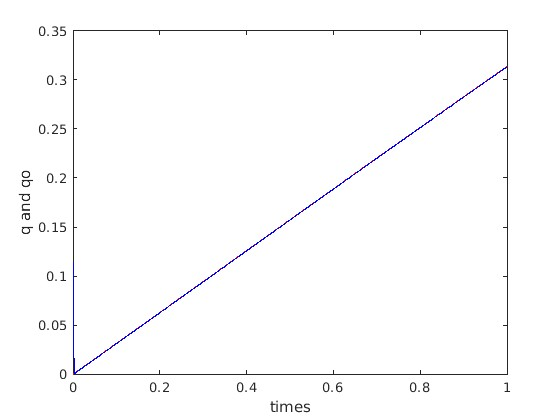
\includegraphics[width=\linewidth]{q_and_qo}
\caption{Aproximación.} \label{fig:aproximacion}
\end{figure}

\begin{figure}[htbp]
\centering
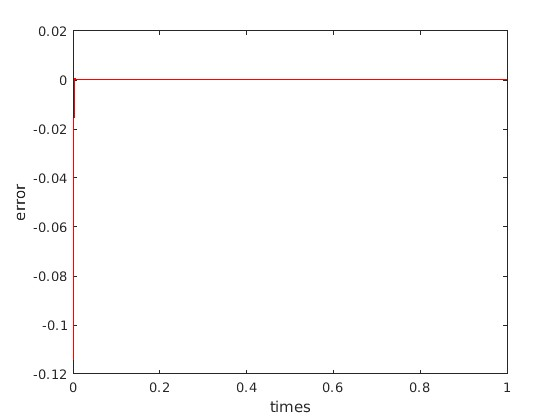
\includegraphics[width=\linewidth]{error}
\caption{Error de aproximación.} \label{fig:error}
\end{figure}

\begin{figure}[htbp]
\centering
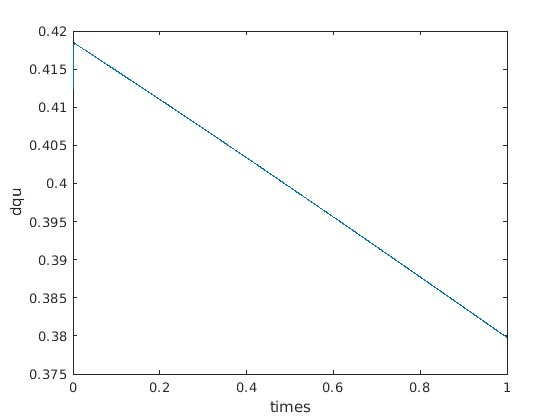
\includegraphics[width=\linewidth]{dqu}
\caption{Jacobiano.} \label{fig:dqu}
\end{figure}

\end{document}


